\documentclass[convert={density=900,size=1080x800,outext=.png}]{standalone}
\usepackage[utf8]{inputenc}
\usepackage{tikz}

\usetikzlibrary{calc, positioning}
\usetikzlibrary{arrows.meta}
\usetikzlibrary{matrix}
\usetikzlibrary{shadows}
\usepgflibrary{shapes.misc}
\usepgflibrary{{shapes.geometric}}

\pgfdeclarelayer{shadow} 
\pgfsetlayers{shadow,main}
\def\shadowradius{3pt}


\def\mw{2cm}
\def\mh{1.75cm}
\def\trianglecoordinate{2mm}

\newcommand\drawshadowbis[1]{
    \begin{pgfonlayer}{shadow}
        \fill[inner color=black,outer color=white] ($(#1.south west)$) circle (\shadowradius);
        \fill[inner color=black ,outer color=white] ($(#1.north west)$) circle (\shadowradius);
        \fill[inner color=black ,outer color=white] ($(#1.south east)$) circle (\shadowradius);
        \fill[inner color=black,outer color=white] ($(#1.north east)$) circle (\shadowradius);
        \fill[ top color=black, bottom color=white] ($(#1.south west)+((0,-\shadowradius)$) rectangle ($(#1.south east)$);
        \fill[left color=black,right color=white] ($(#1.south east)$) rectangle ($(#1.north east)+((\shadowradius,0)$);
        \fill[bottom color=black,top color=white] ($(#1.north west)$) rectangle ($(#1.north east)+((0,\shadowradius)$);
        \fill[right color=black,left color=white] ($(#1.south west)$) rectangle ($(#1.north west)+(-\shadowradius,0)$);
    \end{pgfonlayer}
    }

\tikzstyle{component} = [draw, fill=white, minimum width=\mw, minimum height=\mh, align=center]

\tikzset{
    border/.style = { 
        draw, rectangle, minimum width=\mw, minimum height=\mh, thick, align=center
    },
    Component/.pic = {
        \node [border, font=\large](-edge){#1}; 
        \draw[thick] ([xshift=\trianglecoordinate] -edge.south) -- ([yshift=\trianglecoordinate] -edge.south);
        \draw[thick] ([xshift=-\trianglecoordinate] -edge.south) -- ([yshift=\trianglecoordinate] -edge.south);
        \draw[thick] (-edge.south) |- ++(-3mm, -4mm) node[xshift=-2mm, yshift=-1mm] {T}; 
    },
}

\tikzset{
    clockborder/.style = { 
        trapezium, trapezium angle=60, minimum width=1cm, draw, very thick
    },
    Clock/.pic = {
        \node [clockborder, shape border rotate=-180](-clockedge){#1};
        \draw[very thick] (-clockedge.east) -- ++(2cm, 0cm);
        \def\sft{0.5}
        \foreach \x in {0, 0.5, 1, 1.5}{
            \draw[very thick] (\x + \sft, 0.1) -| ++(0.25cm, 0.25cm) -| ++ (0.25cm, -0.25cm);
        }
    },
}

\begin{document}
    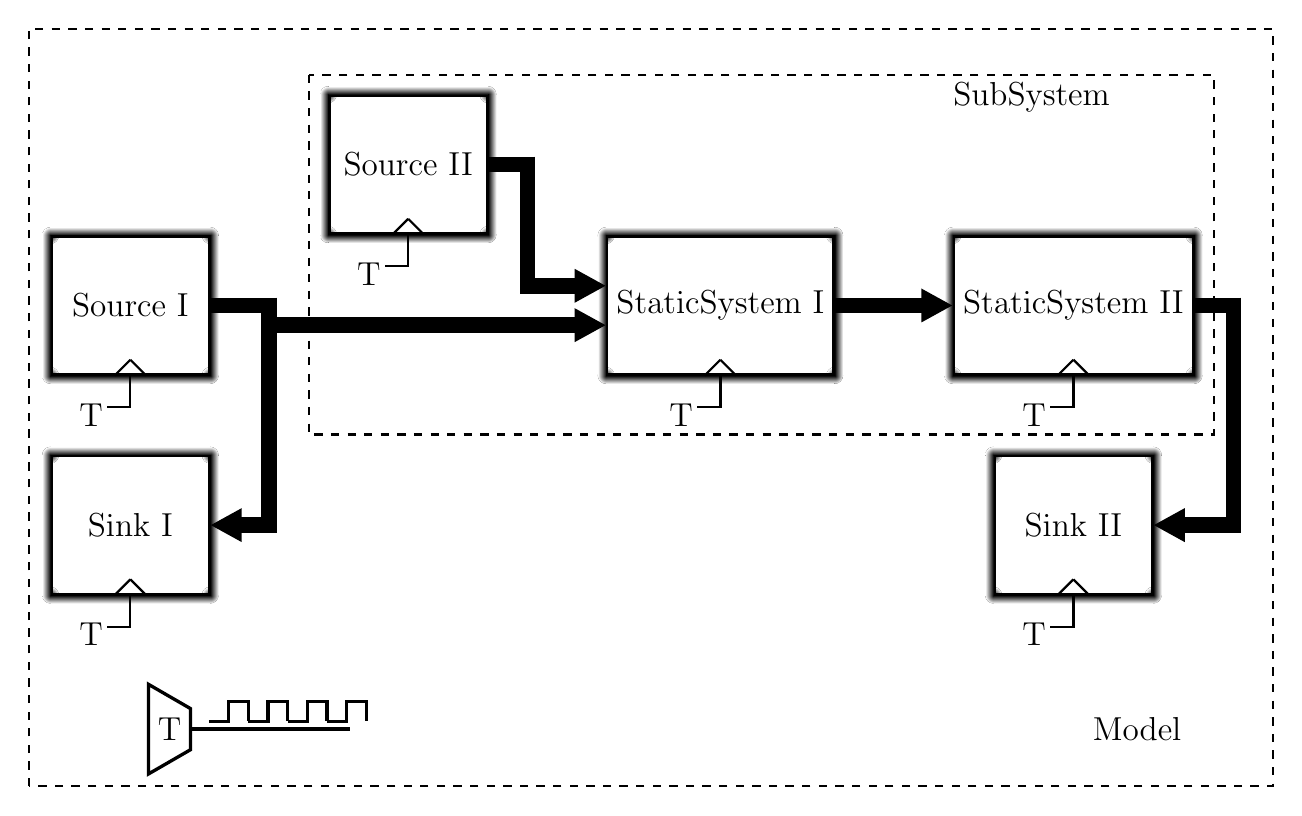
\begin{tikzpicture}[every node/.style={font=\large}]
        % Place the blocks 
        \matrix (m) [matrix of nodes, ampersand replacement=\&, column sep = 1.5cm, row sep = 0.25cm, nodes={anchor=center}]{
             \& \draw pic (kaynak2) {Component={Source II}}; \& \&   \\[-1cm]
            \draw pic (kaynak1) {Component={Source I}};    \& \& \draw pic (statiksistem1) {Component={StaticSystem I}}; \& \draw pic (statiksistem2) {Component={StaticSystem II}}; \\
            \draw pic (kutuk1) {Component={Sink I}}; \& \& \& \draw pic (kutuk2) {Component={Sink II}}; \\
        };
        % Glow the blocks
        \foreach \x in {kaynak1, kaynak2, kutuk1, kutuk2, statiksistem1, statiksistem2}{
            \drawshadowbis{\x-edge};
        }
        % Draw connections 
        \begin{scope}[line width=2mm, >={Triangle[width=4mm,length=4mm]}]
            \draw[-] (kaynak1-edge.east) -- ++(0.75cm, 0cm) coordinate(a);
            \draw[->] ([yshift=1mm] a) |- (kutuk1-edge.east);
            \draw[->] (a) |- ([yshift=-0.25cm] statiksistem1-edge.west);
            \draw[-] (kaynak2-edge.east) -- ++(0.5cm, 0cm) coordinate(b);
            \draw[->] ([yshift=1mm] b) |- ([yshift=0.25cm] statiksistem1-edge.west);
            \draw[->] (statiksistem1-edge.east) |- (statiksistem2-edge.west);
            \draw[-] (statiksistem2-edge.east) -- ++(0.5cm, 0cm) coordinate(c);
            \draw[->] ([yshift=1mm] c) |- (kutuk2-edge.east);
        \end{scope}

        % Draw rectangle for subsystem 
        \draw[thick, dashed] ([xshift=-0.25cm, yshift=0.25cm] kaynak2-edge.north west) rectangle ([xshift=0.25cm, yshift=-0.75cm] statiksistem2-edge.south east);
        \draw (statiksistem2-edge.north west) node[yshift=1.75cm, xshift=1cm]{SubSystem};

        % \Place clock 
        \begin{scope}[shift={(-5.75cm, -4.5cm)}]
            \draw pic(clk) {Clock={T}} ;
        \end{scope}

        %  Draw rectangle 
        \draw[dashed, thick] ([xshift=-0.75*\mw, yshift=-0.25*\mh] clk-clockedge.south west) rectangle ([xshift=0.5*\mw, yshift=1.5*\mh] statiksistem2-edge.north east);
        \draw (clk-clockedge.east) node[yshift=0*\mh, xshift=6*\mw]{Model};
    \end{tikzpicture}
\end{document}